\newpage
\chapter{Related Work}


In diesem Kapitel werden die Grundlagen erläutert und bereits bekannte Implementierungen erklärt.  Das Kapitel beginnt mit einer kurzen Übersicht über die Funktionsweise von Datenbanksystemen vor dem Hintergrund der Anfrageoptimierung. Im Zentrum stehen die Komponenten Query Optimizer und Query Execution Engine. Beide Teile sind integraler Bestandteil eines Datenbanksystems. Im weiteren wird der für die Anfragenoptimierung wichtige Begriff des Search Spaces eingegangen. Das Kapitel wird fortgesetzt mit einer Übersicht über bereits bestehende Datenbanksysteme und deren Optimierer. Es wird konkret auf IBMs Starburst-Projekt und das EXODUS Projekt \cite{graefe1987exodus}, \cite{carey1990exodus} mit seinen Nachfolgern Volcano \cite{graefe1990parallelizing}, \cite{graefe1990encapsulation}, \cite{graefe1993volcano}, \cite{graefe1994volcano} und Cascades \cite{graefe1995cascades} eingegangen. Abgerundet wird das Kapitel mit einer Erklärung der von Pellenkoft zusammengestellten Regelsets \cite{pellenkoft1997complexity}, \cite{pellenkoft1997duplicate}. Alle Komponenten zusammen bilden die Grundlage für die im nächsten Kapitel besprochene Implementierung der Planexpanders.


\section{Historischer Überblick}
Der Grundstein für Anfragenoptimierung wurde durch System R gelegt. Das System beinhaltet einen Algorithmus, der mit Hilfe von dynamischer Programmierung, eine optimale Join Order für eine Anfrage bildet. Das System prägte auch das Konzept der Interesting orders for exploiting available ordering. Bei späteren System wurde die Menge der optimierten Operatoren weiter vergrössert und regelbasierte Optimierungstechiken eingeführt. Ein Beispiel für dieses Systeme ist Starburst, das im folgenden weiter besprochen wird, es ist die weiterentwicklung von System R bei IBM und ist der Prototyp für DB2. Starburst bekann meherere Interne Repräsentationen der Anfrage einzuführen genauso wie Grammer-like Regeln zur Kombination von LOLEPOPs in Execution Plans. Ähnlich wie System R nutzt es einen Buttom-up Approach. Eine andere Familie an Optimierern fusst auf der Arbeit an EXODUS, aus dem Volcano und schliesslich Cascades entsand. Im gegensatz zu dem Bottom-up approach nutzt Voplcano einen Transformaiven Top down optimierungs Ansatz mit Memorization. 



\subsection{System R}

System R ist ein von IBM in den 1970er Jahren durchgeführtes Datenbank Research Projekt \cite{selinger1979access}, \cite{wade2012ibm}, \cite{chamberlin1981history}, \cite{astrahan1976system}, \cite{astrahan1978system}. Es gilt insbesondere auf Grund von zwei Aspekten als der Pinoneer für moderne Datenbanksysteme: Auf der einen Seite wurde in System R zum ersten Mal \ac{SQL} implementiert. Auf der anderen Seite war es das erste System, das die Leistungsfähigkeit von relationalen Datenbanksystemen unter Beweis stellte. Fundamentale Design Entscheidungen, wie dynamische Programmierungsalgorithmen für \ac{QO}, prägen die weitere Entwicklung von Datenbanksystemen. System R gilt als der Vorgänger von IBMs DB2 und als Grundlage für viele andere Datenbanksysteme.


\subsubsection{Architektur und Systemstruktur}

\begin{figure}[h]
  \centering
  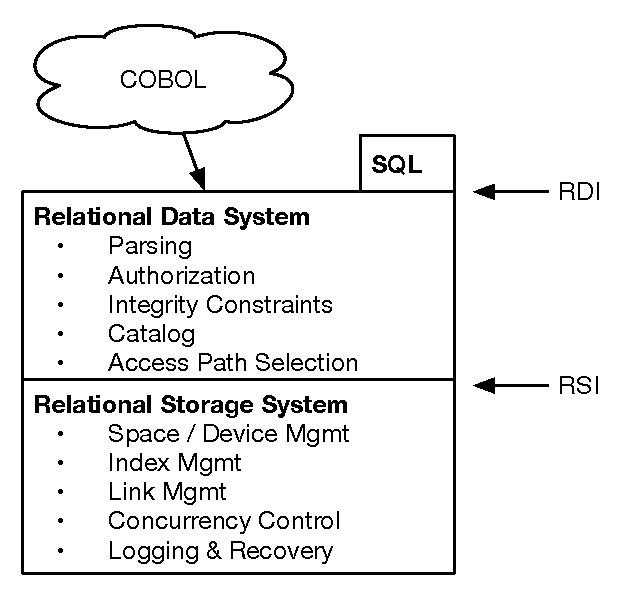
\includegraphics{03_Related_Work/SystemR.pdf}
  \caption{System R Architektur \cite{astrahan1976system} \cite{astrahan1978system}}
  \label{SystemRArchitecture}
\end{figure}


Wie in Abbildung \ref{SystemRArchitecture} zu erkennen ist,  besteht das System aus zwei Teilsystemen: \ac{RSS}, das dem RTS entspricht, und \ac{RDS}, das äquivalent zu einem CTS ist.

Das \ac{RSS} ist für die physische Verwaltung der Datenbank verantwortlich. Es kontrolliert u.a. die Speicherverwaltung, das Device-Management, die Transaktionskonsistenz und die Transations- sowie System-Wiederherstellung. Im Besonderen fällt in den Aufgabenbereich der Zugriff auf einzelne Tupel von Base Relations. Diese Funktionen werden gegenüber des \ac{RDS} mit Hilfe des \ac{RSI} bereitgestellt.

Das \ac{RDS} übernimmt via \ac{RDI} die Kommunikation nach außen und leitet Befehle über das \ac{RSI} weiter. Anfragen von außen werden mit Hilfe von \ac{SQL} an das System gestellt. Es ist auch möglich, dass externe Sprachen wie Cobol verwendet werden, die ohne Weiteres mit dem \ac{RDI} kommunizieren. In diesen Fällen muss SQL nicht verwendet werden. Das \ac{RSS} wandelt die Umfrage in eine für das \ac{RSI} verständliche Form um. Über das RSI wird die Anfrage entgegen genommen und ausgeführt.




\subsubsection{Verarbeitung von Anfragen}

Wie bei anderen relationalen Datenbanksystemen steht am Beginn eine in \ac{SQL} formulierte Anfrage. Diese Anfrage wird in vier Schritten verarbeitet: Parsen,  Optimieren, Code Generierung und Ausführen.

Im ersten Schritt, Parsen, wird wie bei späteren Systemen die Syntax geprüft und die Anfrage in eine interne Repräsentation umgewandelt. Bei System R werden hierzu Query Blöcke verwendet. Sie repräsentieren die Anfrage mit einer SELECT list, einer FROM list und einem WHERE Baum. Er beinhaltet eine Liste der Elemente, die beispielsweise zum JOIN von Tabellen und der Einschränkung von Datensätzen dienen. Es ist möglich, dass mehrere Query Blöcke für eine einzige Anfrage vorhanden sind. Dies geschieht dann, wenn eine Anfrage Inner-Queries verwendet bzw. Anfragen als Argumente für eine WHERE Bedingung zum Einsatz kommen.


Sobald die Anfrage in Query Blöcke verarbeitet wurde, kommt der \ac{QO} zum Einsatz. Der Optimierer prüft zuerst, ob die genutzten Relationen und Felder auch in der Datenbank vorhanden sind und schlägt Informationen über diese im System R Catalog nach. Teil dieser Informationen sind statistische Informationen der referenzierten Relationen. Diese werden später für die Auswahl der richtigen Access Plans verwendet.

Im nächsten Schritt, optimieren, bestimmt der Optimizer für jeden Query Block den optimalen Access-Pfad. Zuerst wird die Evaluationsreihenfolge der Query Blocks im Statement festgelegt. Dann wird für jeden Query Block die FROM Relationen betrachtet. Sind mehr als eine Relation vorhanden, werden Permutationen der JOIN-Order gebildet. Es wird der Pfad mit den günstigsten Kosten gewählt und die notwendigen Modifikationen werden an der Anfrage vorgenommen. Das Resultat des Prozesses ist ein Plan in der \ac{ASL}.

Nachdem der Plan gefunden und als \ac{ASL}-Tree vorhanden ist, kommt der Code Generator zum Einsatz. Er übersetzt den \ac{ASL}-Plan in einen  Maschinencode. Dieser Code führt die Anfrage des Nutzers auf der Datenbank aus. 

Der Maschinencode wird dann auf dem \ac{RSS} über das \ac{RSI} ausgeführt und das Ergebnis zurückgegeben.

\subsubsection{Kostenberechnung}
Bei der Auswahl des optimalen Plans beginnt System R mit der Reihenfolge der Query Blocks. Zuerst wird für jeden Query Block geprüft, ob mehrere Tabellen in den FROM Listen vorhanden sind. Falls das der Fall ist, wird die Optimale Join-Order und die Methode des Joins bestimmt. Der Plan mit den geringsten Gesamtkosten für einen Block wird ausgewählt.

Zur Bestimmung der Kosten werden statistische Informationen aus dem System R Catalog herangezogen. Die Berechnung der Kosten für einen Access Plan, werden mit Hilfe der folgenden Funktion abgeschätzt:

$$Cost = Page Fetches + W * (RSI calls)$$


$Page Fetches$ repräsentieren die I/O Operationen, die beispielsweise durch den Abruf der Index Pages und der eigentlichen Pages entsteht. $RSI calls$ ist die Anzahl der erwarteten Datensätze, die durch das \ac{RSS} zurückgegeben werden. Sie dient als Abschätzung wie hoch der CPU Aufwand für die Rückgabe der Werte ist. Mit Hilfe des Parameters $W$ wird eingestellt in welchem Verhältnis I/O zu CPU Kosten stehen.


%\sout{Bei der Auswahl eines Plans unterscheidet das System zwischen einer \"interessanten\" Reihenfolge, also sortierten Ergebnissen, und einer ungeordneten Reihenfolge. Als interessante Reihenfolge, werden Reihenfolgen betrachtet, die gesamter Reihenfolge notwendig sind und die Kosten, die für das lesen in ungeordneter Reihenfolge notwendig sind und addiert auf diese Kosten, die Kosten für das Ordnen der Ergebnisse falls eine ungeordnete Reihenfolge + das Ordnen der Ergebnisse gemeinsam kürzer dauert als das direkte Ausgeben einer interessanten Reihenfolge wird sich für die günstigere Variante entschieden.}


Die Berechnung findet auf Basis der Daten statt, die von System Rs Catalog bereitgestellt werden. Die Daten umfassen folgende Kennzahlen:

\begin{itemize}
\item $R$: Kardinalität der Relation (Anzahl Tupel)
\item $D$: Anzahl der Daten-Pages, die von der Relation belegt werden
\item $T$: Durchschnittliche Anzahl der Tupel pro Daten Page (gleich $G/D$).
\item $H$: Koeffizient der CPU-Kosten ($1/H$ ist die Anzahl der Tupelvergleiche, die  als gleich den Kosten für einen Page Access sind.)
\end{itemize}

Auf Basis dieser Kennzahlen werden die Kosten je nach Operator festgestellt. 

%\sout{Die Berechnung geschieht auf Daten, die durch den Catalog bereitgestellt werden, Sie enthalten Informationen über die Kardinalität und die Anzahl der Segmente, die für das auslesen einer Relation notwendig sind, ebenfalls wird ein Selektivitätsfaktor genutzt, der das Verhältnis der Gesamtheit zur eingeschlossenen Menge der Anfrage angibt. Sprich die Menge der ausgeschlossenen Tupel.}



\subsubsection{Plan Enumerator}
Die Enumeration des System R Optimizers zeigt zwei wichtige Aspekte eines Enumerators: Auf der einen Seite die    interesting order  auf der anderen Seite  die \"dynamic Programming\". 

Dynamische Programmierung geht davon aus, dass das Kostenmodell dem Optimalitätsprinzip von Bellman \cite{Bellman:1957} gehorcht. Das Prinzip sagt aus, dass sich eine Optimallösung aus optimalen Teillösungen zusammensetzt. In unserem konkreten Fall sagt das Prinzip, dass der optimale Plan nur aus optimalen Teilbäumen bestehen kann. Somit müssen nur optimale Subplans zur Erzeugung des optimalen Plans verwendet werden i.a.w. sucht man mit Hilfe eine bottom-up Enumeration Algorithmus nach dem optimalen Plan. So müssen nur Subpläne in Betracht für eine optimale Gesamtlösung gezogen werden, die für sich optimal sind. 

Ein weiterer wichtiger Aspekt von System R ist die Verwendung von Interesting Orders. Als Interesting Orders werden Reihenfolgen, die innerhalb eines Joins entstehen bezeichnet, die zwar höhere direkte Kosten verursachen, jedoch zu niedrigeren Gesamtkosten beitragen können. So ist es möglich, dass die Kosten durch einen Nested-Loop Join zwar höher sind als durch einen Merge-Join, allerdings die Gesamtkostenbilanz durch den teureren Nested-Loop Join positiv beeinflusst wird. Gerade beim Einsatz von Prunning Algorithmen ist es möglich, dass so ein global suboptimaler Plan gewählt wird. System R identifiziert diese geordneten Resultate, die für die zukünftige Ausführung von Vorteil sein können. Außerdem werden Pläne in System R nur dann verglichen, wenn sie die selbe Reihenfolge und den selben Ausdruck besitzen. 


\section{Das Starburst Project}

Das Starburst Projekt \cite{lohman1988Starbust}, \cite{haas1989extensible}, vorangetrieben und entwickelt von IBM,  startet unter der Prämisse, dass bestehende DBMSe nicht in der Lage sind die wachsenden Anforderungen von verschiedenen, neuartigen Applikationen vollumfänglich zu entsprechen. Zur Erfüllung der individuellen Ansprüche wurde das Starburst Projekt begonnen. Sein Ziel ist es dem \ac{DBI} die Möglichkeit zu geben eine die relationale Datenbank zu erweitern und so die Bedürfnisse von spezifischen Anwendungen zu erfüllen. Beispielsweise ist es möglich neue Zugriffs- und Speichermethoden zu implementieren oder neue Join Methoden zu erstellen. Um diese Features zu ermöglichen stellt Starburst eine Anfragesprache, einen regelbasierten Optimierer, Query Rewriter und ein Ausführungssystem basierend auf relationaler Algebra zur Verfügung. Dieses Kapitel befasst sich zuerst mit der Aufteilung zwischen Ausführung und Anfrage, wie sie bereits zu Beginn dieses Kapitels besprochen wurde. Es folgt ein Überblick über die eingesetzte Regelmaschine und eine Erläuterung des Starbust Query Optimizers.

\subsection{Ausführung einer Anfrage}

Bei der Ausführung einer Anfrage mit Hilfe von Starburst wird grob zwischen zwei Phasen unterschieden: Übersetzungs- (Compile-) und Ausführungszeit (Run-Time). Während der Compile-Time wird aus der Anfrage ein Plan generiert, der zur Run-Time durch das Execution System ausgeführt wird. Der Query Optimizer findet seine Anwendung zur Compile-Time; die Query Execution Engine kommt zur Run-Time zum Einsatz.

\begin{figure}[h]
  \centering
  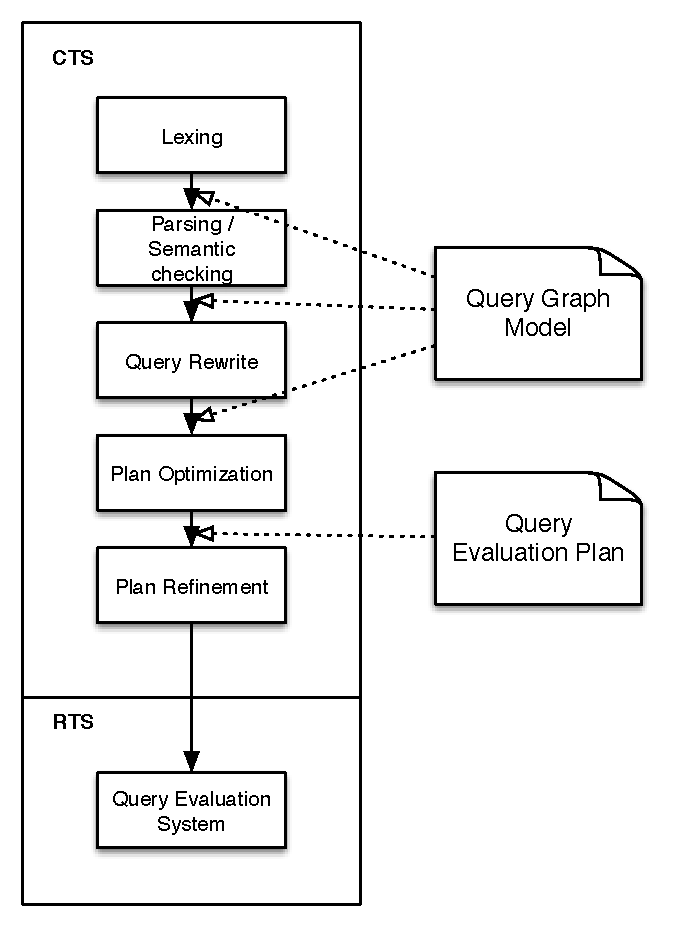
\includegraphics{03_Related_Work/StarburstFlow.pdf}
  \caption{Starburst}
\end{figure}

Zur Comile-Time wird eine gegebene Anfrage auf semantische Korrektheit geprüft und in ein \ac{GQM} übersetzt. Basierend auf diesem \ac{GQM} wird die Optimierungen der Anfrage durch zuerst einen Query Rewriter, einen Plan Optimierer und einen Plan Refiner durchgeführt.

Der Query Rewriter hat zwei konkrete Aufgaben: Auf der einen Seite soll die Anfrage in eine möglichst deklarative Form umgewandelt werden, hierbei werden insbesondere Anfragen entschachtelt. Auf der anderen Seite sollen weithin in der Forschung akzeptierte Heuristiken, beispielsweise der Push-Down von Argumenten, angewandt werden.
Bei der Planoptimierung durchläuft der Plan vom \ac{GQM} hin zu einem QEM drei Stationen. Die drei wesentlichen Aspekte sind der Plan Generator, die Berechnung der Plankosten, um den optimalen Plan auszuwählen. 

\subsection{Regel-Maschine}

Zur Ausführung von Optimierungen wurde für die Starburst Datenbank eine eigene Regel-Maschine entwickelt \cite{lohman1988Starbust}. Diese Regelmaschine ist für die Anführung von Regelsets verantwortlich, die bei der Transformation der QGMs zur Anwendung kommen und durch den \ac{DBI}  erweitert werden können. Die Regelmaschine basiert auf fünf Prinzipien:

\begin{enumerate}
\item Regel der arbiträren Komplexität: Eine Regel ist bei Starburst in zwei Teile aufgeteilt: Eine Koordinierungs- und eine Ausführungsfunktion. Bei dem Aufruf einer Regel muss zuerst geprüft werden, in wie weit die Regel angewendet werden darf. Ist sie anwendbar, wird die Ausführungsfunktion exekutiert.

\item Bei der Nutzung eines GQMs kann entweder eine Tiefen- als auch eine Breitensuche zur Anwendung kommen. Diese Art der Suche ist weder an die Regel noch an das Regel-Set geknüpft, sondern mit dem QGM selbst verbunden.


\item Die Regeln werden bei Starburst in Regelsets unterteilt. Ein Regel-Set besteht aus mehreren Regeln, die entweder sequenziell, nach einer vorab vergebenen Priorität oder einem statistischen Verfahren aufgerufen werden. Jede Regel und jedes Regel-Set kann andere Regeln und Regel-Sets als Teil einer Subroutine ausführen. Neben der Funktion der Zusammenfassung der Regeln ist es Aufgabe der Regel-Sets.

\item Um die Ausführung von Transformationen zu limitieren, insbesondere bei der Ausführung des Rewriters, kann ein Budget vorgeschrieben werden. Sobald dieses Zeitbudget aufgebraucht ist, wird die Ausführung von Transformationsregeln abgebrochen. Es ist für diese Funktion unbedingt notwendig, dass Regeln immer vollständige QGMs zurückliefern, da sonst ein unvollständiger QGM als Resultat des Optimierers entstehen kann.

\item Schlussendlich ist es dem Nutzer der Datenbank möglich zu jedem beliebigen Zeitpunkt Regeln ausser Kraft zu setzen. Dies geschieht nur für den Nutzer lokal und andere Nutzer der Datenbank sind nicht betroffen. Spezielle Anwendungsfälle können so passgenau optimiert werden.
\end{enumerate}

\subsection{Plan Optimierer}

Der Plan Optimierer generiert basierend auf einem QGM mehrere alternative Query Evaluation Plans (QEPs). Für jeden dieser QEPs werden die Kosten geschätzt und der günstigste für die Weiterverarbeitung ausgewählt. Um die Erweiterbarkeit des Optimierers zu gewährleisten wurden die drei Komponenten (Plangenerierung, Kostenschätzung und Suchstrategie) von einander soweit getrennt, dass sie einzeln erweitert und verändert werden können. 

\subsection{Starburst Plan Generator}
\emph{HIER ÜBERARBEITEN}
Der Plangenerator des Starburst Projekts, der für die Generierung von Planalternativen verantwortlich ist, bedient sich eines "Build Block"-Ansatzes[Lohm88] und einem Regel-Set, das auf einer eigenen Grammatik basiert.  

Als Build Block werden low-level-Datenbankoperationen (wie Access, Join und Sort) zu high-level Operationen kombiniert. Diese können wiederverwendet werden. Dank des Konzepts der Build Blocks ist es möglich die Erstellung und Verarbeitung in zwei wesentlichen Aspekten zu vereinfachen:


\begin{enumerate}


\item Die Regeln sind leichter von einem DBI zu lesen und zu verstehen, da die Fülle an Information mit Hilfe von Build Blocks aggregiert wurde.

\item Das Ausführen von Regeln wird effizienter. Da nicht mehr ganze Graphen nach Pattern durchsucht werden müssen, sondern direkt über Build Blocks erkannt werden, erleichtert sich die Ausführung. Ebenfalls ist es dank der Nutzung von Macro-Expandern möglich, die Geschwindigkeit zu verbessern.


\end{enumerate}


$$TEXT$$
Jede Regel erlaubt es, dass aus ihr sowohl eine als auch mehrere Graphen entstehen können. In diesem Falle spricht man von Sets von Alternativen Plänen (SAP). 


\begin{itemize}
\item LOLEPOP
\item STARs
\end{itemize}

 

\subsection{Exodus, Volcano, Cascades}

In diesem Kapitel wird der Verlauf des EXODUS Projektes und seiner Nachfolger Volcano und Cascades behandelt. Zuerst wird ein allgemeiner Überblick über den Aufbau von EXODUS gegeben. Hierauf werden die Änderungen und Erweiterungen von Volcano und Cascades besprochen. Insbesondere wird in diesem Teil auf die Art und Weise der Implementierung der Query Optimizer eingegangen. 

\subsubsection{Exodus}


Bereits in den 1970er Jahren begann Graefe mit der Implementierung eines DBMS Frameworks unter dem Titel EXODUS (EXtensible Object-oriented Database System) \cite{carey1990exodus} . Das Projekt, das die Grundlage für Volcano legen sollte, hatte sich zum Ziel gesetzt einen erweiterbaren, applikationsspezifischen und hochperformanten Baukasten zusammenzustellen, mit dessen Hilfe neue Datenbanksysteme generiert werden konnten. 

Im Gegensatz zu konventionellen DBMS wie Postgres handelt es sich bei EXODUS nicht um ein funktionsfähiges und sofort einsatzfähiges DBMS, sondern um einen Baukasten, auf dessen Basis ein neues System durch einen DBI erstellt werden kann. Im Gegensatz zu anwendungsübergreifend designten DBMS wie Postgres bietet EXODUS den Vorteil, dass eine Datenbank speziell für die Bedürfnisse eines Anwendungsfalles angepasst wird. Um dennoch das Ziel der Performance nicht aus den Augen zu verlieren, werden viele Komponenten nicht immer wieder auf einer grünen Wiese entwickelt, sondern auf dem Fundament des EXODUS Baukastens aufgebaut.

\begin{figure}[h]
  \centering
  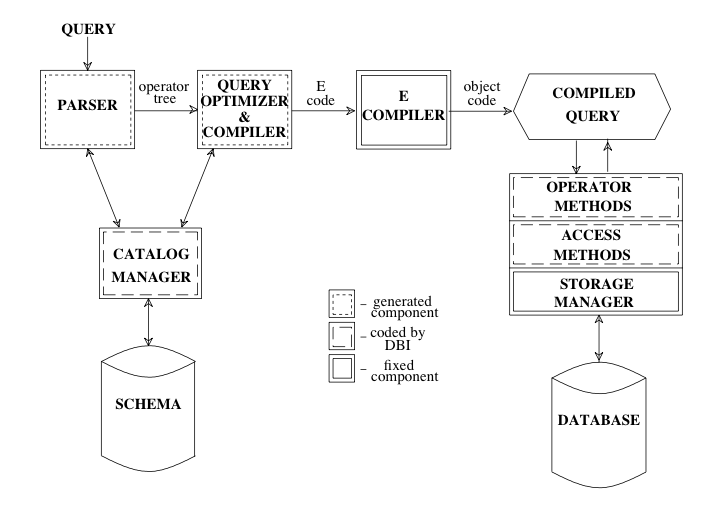
\includegraphics[width=\textwidth]{02_Grundlagen/ExodusDatabaseSystemStructure.png}
  \caption{Exodus Database System Structure}
\end{figure}

Der Baukasten von EXODUS erlaubt       besteht sowohl aus Bestandteilen, die fix vorgegeben und nicht verändert werden sollen, Bausteinen die generiert werden und Teilen, die speziell entwickelt werden müssen. Der Werkzeugkasten umfasst dabei nicht nur die Bausteine, sondern auch die Werkzeuge zur Bearbeitung und Generierung. Zu den Werkzeugen gehören ein Tool zur Erstellung eines Front-Ends für die Anfragesprache, ein Query Optimizer Generator und die Programmiersprache E (zusammen mit einem passenden Compiler). Mit Hilfe des Tools zur Erstellung eines Front-Ends für Anfragesprachen kann die Parser Komponente generiert werden. Der Query Optimizer wird als Resultat des Query Optimizer Generators erzeugt. (vgl. Fig. Exodus Database System Structure)

Neben den generierten Komponenten gibt es den E Compiler, der E Code in Objekt-Code übersetzt. Er kommt zum Einsatz, um die durch den Query Optimizer optimierte Anfrage in eine kompilierte Anfrage umzusetzen. Diese Komponente ist ähnlich wie der Storage Manager, der für die Verwaltung von Daten in der Datenbank genutzt wird unveränderlich. 

Zwischen der kompilierten Anfrage und dem Storage Manager kommen zwei Komponenten zum Einsatz, die von einem DBI geschrieben werden müssen: Die Operator Methoden und Access Methoden. Diese beiden Komponenten dienen dazu die Anfrage in Code zu übersetzen, der durch den  Storage Manager ausgeführt wird.

Bei der Implementierung eines Optimierers kommen grundsätzlich zwei mögliche Ansätze in Frage: (1) interpretierte und (2) kompilierte Programmiersprachen. Bei EXODUS wurde zuerst die Implementierung mittels sog. "AI" Sprachen versucht. In einem Prototypen wurde mit Hilfe von Prolog ein Optimierer entwickelt. Für Prolog wurde sich entschieden, da diese Sprache Pattern Matching und eine Search Engine bereitstellt. (Auch unification konnte zum Einsatz gebracht werden, um elegant Query Trees zu erstellen.) Der Hauptvorteil eines interpretierten Ansatzes war aus Sicht von EXODUS die Möglichkeit neue Regeln zur Laufzeit des Programms hinzuzufügen. Trotz dieser Vorteile wurde der Ansatz als zu langsam verworfen. Auch der Vorteil Regeln während der Laufzeit hinzuzufügen, wird in der Literatur (QUELLE) als wenig nützlich bewertet. Statt dieses Ansatzes wurde in der Folge auf die Erstellung eines Generators, der in C geschrieben wurde, gesetzt. Der Generator erstellt basierend auf Regeln einen Optimierer in C, der wiederum kompiliert werden kann. Zwar war die Entwicklung des C Generators aufwendiger als die Implementierung in Prolog, jedoch konnte auf applikationsspezifische Notwendigkeiten, wie die Implementierung von speziellen Suchverfahren, Punkt genau eingegangen werden.


Der generierte Optimierer funktioniert so, dass er den Anfragenbaum Schritt für Schritt transformiert. Die Information über bereits erstellte Baum-Alternativen wird in einer Datenstruktur namens MESH gespeichert. MESH wird außerdem genutzt um Plänge für Anfragenbäume zu speichern, die nicht beschnitten werden von der Daten Struktur. Zu jedem Zeitpunkt während der Optimiererung kann eine große Menge an weiteren möglichen Transformationen. Diese wird in der Datenstruktur \"OPEN\" gespeichert. Sie ist eine Priority Queue. OPEN ist initalisiert mit Transformationen, die auf den initialen Tree angewendet werden können. Grundsätzlich funktioniert der Algorithmus wie folgt:

\begin{lstlisting}[caption={Exekution in EXODUS}]
While (OPEN is not empty)
	SELECT a transformation from OPEN
	Apply it to the correct node(s) in MESH
	DO method selection and cost analysis for the new nodes
	Add newly enabled transformations to OPEN

\end{lstlisting}

\subsubsection{Volcano}

Volcano ist der verbesserte Nachfolger von EXODUS. Zuerst war Volcano nur ein erweiterbares, paralleles System zur Anfragenausführung. Später wurde ein neuer Anfragenoptimierer-Generator hinzugefügt. 

Der Volcano-Optimizer-Generator wurde designt und implementiert 





\subsubsection{Volcano Optimizer Generator}

Der Volcano Optimizer unterscheidet sich verglichen zu seinem Vorgänger EXODUS durch höhere Erweiterbarkeit. Er bietet Unterstützung für nicht triviale Kostenmodelle und physische Eigenschaften wie die Sortierreihenfolge von Relationen. Außerdem ist er effizienter durch die Kombination von dynamischer Programmierung, zielgerichteter Suche und “Branch-and-Bound-pruning.” Im Vergleich zu anderen regelbasierten Optimieren ist das System unabhängig von einem gegebenen Datenmodell.

\subsubsection{Volcano Optimizer Generator}

Bei der Generierung eines Plans auf Grund einer Anfrage kommt bei Volcano ein Optimierer zur Anwendung, der speziell für den Anwendungsfall generiert wurde. Der Optimierter ist das Resultat einer Model Spezifikation, die von einem Datenbank Implementierer (DBI) erstellt und durch einen Optimierer Generator in Source Code umgewandelt wird. Dieser Code wird mit Hilfe eines Compilers in das Endprodukt, den Optimierer, umgewandelt.

 \subsubsection{Design Prinzipien}

Der Optimierer folgt dabei fünf Designentscheidungen \cite{graefe1993volcano}, die die Erweiterbarkeit und eine Effiziente Suche des Optimiers erlauben.

\begin{itemize}

\item Die erste Grundlage des Volcano Optimizers ist die Anwendung von algebraischen Techniken wie algebraische Operatoren und Äquivalenzklassen. Volcano unterscheidet dabei zwischen logischer und physischer Algebra. Die Umwandlung von logischer Algebra (der Anfrage) in die physische Algebra (einem Query Evaluation Plans) geschieht bei durch die Transformation der logischen Algebra mit Hilfe von kostenbasierten Mappings von Logischen Algorithmen.


\item Das zweite Prinzip sieht vor, dass die Information über algebraische Gesetze, die zur Transformation von Algebraischen Ausdrücken genutzt werden als Regeln und Pattern modular erfasst sind. Durch dieses Prinzip sind die einzelnen Regeln klar und transparent von einander getrennt und können zu Regelsets zusammengestellt werden. Einige dieser Regelsets werden im folgenden Kapitel behandelt.


\item Das dritte Prinzip betrifft den Input des Optimierers im Gegensatz zu anderen Optimierern (namentlich Stardust) setzt der Volcano Optimizer auf algebraische Äquivalenzen als Input Parameter. Andere Systeme nutzen hier mehrere Stufen an Umwandlung, um zwischen Query und Optimizer Input zu vermitteln. 

\item Kompilierung über Interpretierung von Regeln ist das vierte Prinzip, das zur Anwendung kommt. Da es sich bei der Generierung von äquivalenten Plänen um ein CPU intensives Geschäft handelt, wurde entschieden, dass die Regeln zur Transformation der Pläne kompiliert und nicht interpretiert werden. Zwar verliert der Optimierer daduch die Möglichkeit ad hoc neue Regeln in den Optimierer aufzunehemen. Diese Möglichkeit wird jedoch in der Praxis nicht benötigt.

\item Das letzte Prinzip ist, dass der Volcano Optimierer auf dynamisches Programmieren bei der Generierung von Programmen setzt. 


\end{itemize}







\section{Oracle}
\subsection{Oracle Architektur}


\begin{figure}[h]
  \centering
  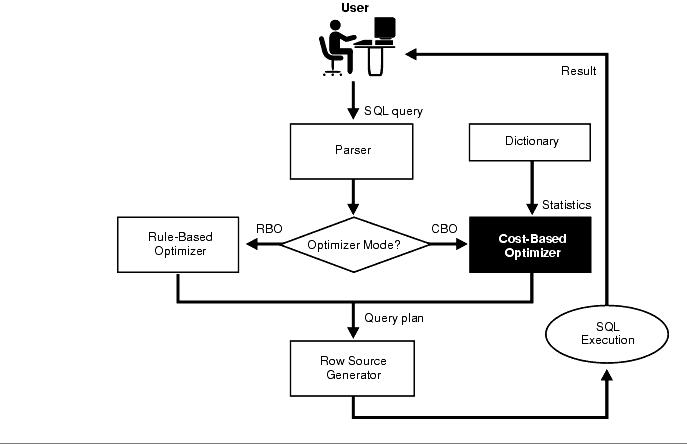
\includegraphics[width=\textwidth]{03_Related_Work/OracleArchitecture.png}
  \caption{Oracle Architecture \cite{Oracle2004Basics}}
  \label{OracleArchitecture}
\end{figure}



Die Oracle Architektur zur Verarbeitung von Anfragen \cite{Oracle2004Basics} (vgl. Abb. \ref{OracleArchitecture})  beginnt wie die meisten Systeme mit einer SQL Anfrage, die von einem Parser in eine Interne Repräsentation gebracht wird. Der Parser übernimmt dabei zwei Funktionen. Auf der einen Seite die Syntaktische Analyse. Es wird geprüft, ob die SQL Anfrage die korrekte Syntax besitzt. Auf der anderen Seite eine Semantische Analyse. Diese prüft beispielsweise ob Datenbank Objekte und Objekt-Attribute  korrekt referenziert werden. Nachdem diese beiden Schritte ausgeführt wurden unterscheidet der Optimierer ob ein \ac{RBO} oder ein \ac{CBO} zum Einsatz kommt. Mit Version 11g der Oracle Datenbank wird der \ac{RBO} nicht mehr unterstützt und ausschließlich auf den \ac{CBO} gesetzt \cite{dba_oracle2015}.

Der \ac{QO} führt bei der Verarbeitung die folgenden drei Schritte aus:

\begin{itemize}
\item Eine Menge potentieller Pläne wird basierend der SQL Anfrage selbst und Hinweisen, die durch den Nutzer eingegeben werden, generiert.
\item Der Optimierer schätzt die Kosten für jeden Plan basierend auf Kosteninformationen über die Anfrage und Storage Charakteristiken der Tabellen, Indexe und Partitionen, die durch ein Statement zugegriffen werden können.

Die Kostenschätzung für den Zugriff auf entsprechende Datensätze und die Reihenfolge der Joins wird nach ihrem Verbrauch von Ressourcen wie I/O, CPU und Memory geschätzt.

Pläne mit höheren Kosten benötigen mehr Zeit zur Ausführung als Pläne mit niedrigeren Kosten. Falls Pläne parallel ausgeführt werden können, ist die Ressourcen Nutzung nicht direkt abhängig von der verwendeten Zeit.

\item Der Optimierer vergleicht die Kosten der Pläne und wählt den kostengünstigsten Plan aus.
\end{itemize}

Das Ergebnis des Optimizers ist ein Plan, der zum Ausführen der Anfrage geeignet ist und als kostenoptimal eingeschätzt wird.


\subsection{Kostenbasierte Transformation in Oracle}

Traditionelle Relationale Datenbank Systeme führen, wie bereits dargestellt, die Transformation von Anfragen in zwei Phasen durch: Logische und physische Phase. In der logischen Phase wird die gegebene Anfrage zuerst durch einen Rewriter angewendet, hier kommen Heueristiken oder Regeln zum Einsatz. Der traditionelle pyhsische Optimizer arbeitet mit einem einzelnen Query Block aus Restriktionen über Tabellen, Projektionen und Joins. Die Physische Optimizerungsphase befasst sich mit Access Methoden, Join Orders und join Methoden die genutzt werden, um effiziente Pläne zu erzeugen.

Query Transformation werden entweder als Rewriter Systeme oder als Extention des Plan generators mit dem pyhsichen Optimierer implementiert. Der erste Ansatz skaliert nicht in komplexen kommerziellen Systemen, der zweite Ansatz ist nur einfach auf ein paar wenige Transformationen anzuwenden. 
Bisher wurden zuerst Rewriter Rules angewendet und dann die Nutzung von Cost Based Trasnformations angewendet. \cite{ahmed2006cost} argumentiert, dass einige Heueristiken nicht immer ein optimales Ergebnis erzeugen und daher mit Hilfe von Cost Based Methoden geprüft werden sollten, bevor sie auf eine Anfrage angewendet werden.


Oracle hat die kostenbasierte Transformation, die logische Transformation und die physische Optimierung kombiniert, um den optimalen Execution Plan zu finden. Der Logische Teil des Systems teilt sich in Heueristiken und kostenbasierte Transformationen. Die kostenbasierten Trasnformatioenen funktionieren wie folgt:

\begin{itemize}
\item Transformationsalorithmen konvertieren gesamte under teil Anfrage Bäume in sequentiell gleiche Form
\item Stae Spaces für verschiedene Transformationen
\item State Space Search Algorithmen
\item Möglichkeit zur Deep Copy von Anfrage Böcken und Ihrer Consitutues
\item Cost estimation techique (physical optimizer)
Transformation derective und cost annotations
\end{itemize}

Unterschiedliche Transformationsregeln werden auf unterschiedliche Teile der Anfrage angewendet. So kann beispielsweise die Entschachtelung nur auf verschachtelte Elemente der Anfrage angewendet werden. 

Die Bäume werden Bottom up transformiert während der Optimierung. Verschiedene Alternativen für eine oder mehrere Transformationen für Elemente in einem Query Tree generieren unterschiedliche States innerhalb des Ste Space of Transformation. Eine Deep kopy wird gemacht bevor ein bestimmter status erreicht wird und dessen Kosten durch den Aufruf des physischen Optimierers geschätzt werden. Die Evaluation von jedem States. Der Transformationsstage, der die besten Kosten bietet wird zurück auf den Ursprungstree angewendet.

Die Oracle Transformationen werden immer hintereinander angewendet. Eine Transformatiosnregel wird immer auf den ganzen Baum angewendet, erst danach folgt die nächste Regel. Die Reihenfolge ist diese: Common sub expression factorization, JPS view merging, join elimination, subquery unnesting, group by distinct view merging, group pruning, predicate move around, set operator factorization, disjunction into union-all exansion, star transfomration and join predicate pushdown. Von dieser Reihenfolge kann jedoch in bestimmten Fällen abgewichen werden. 



\subsubsection{State Space Search Techniques}
Bei der Suche nach einem Plan mit Hilfe von kostenbasierender Transformation stellt sich die grundsätzliche Frage nach einem Trade-off zwischen optimalen Kosten und Execution Kosten. Die Suche nach einer Transformation lohnt sich nur dann, wenn die Kosten für die Suche nach einer besseren Transformation gemeinsam mit der Ausführung der eigentlichen Anfrage geringer ist als die bisher gefundenen Pläne.

Die Frage nach diesem Problem stellt sich insbesondere, wenn eine große Menge an möglichen alternativen Plänen bestehen.. Existieren viele einzelne Objekte einer Anfrage, seien es Query Blocks, Tables join edges predikate, gibt es auch die Möglichkeit, dass viele Regeln auf die Objekte angewendet und somit viele alternative Pläne erzeugt werden können. Wenn $N$ Objekte vorhanden sind und auf diese $N$ Objekte eine Transformation $T$ angewendet wird, dann werden nur durch diese eine transformation $2^N$ verschiedene Pläne generiert. Dies Menge wächst weiter, wenn mehrere Transformationen auf die bestehenden Objekte angewendet werden können. 


Um dieses kombinatorische Problem der vielen oin permutationen zu lösen wurden mehrere randomizierte Algorithmen vorgeschlagen. Tabu Search, Genetic Search, Iterative Improvement...

chst mit der Anzahl der Trasnfromationsobjekte. Wenn die Anzahl der Transformationsobjekte klein ist, dann ist eine enumerative Transformationstechnik mit Hilfe Exhaustive search des States vielleicht machbar. Da aber die Anzahl der möglichen Optimierungen mit der Zeit steigt, müssen andere Techniken angewendet werden:

\begin{itemize}
\item 
\end{itemize}

\subsubsection{Subquery Entschachtelung}

\subsubsection{Join Elimination}

\subsubsection{Filter Predicate Move Around}

\subsubsection{Group Pruning}


\section{Pellenkoft Rulsets}

Bei der Erforschung eines Search Spaces kommen in regelbasierten \ac{QO} Transformationsregeln zum Einsatz. Pellenkoft et al. \cite{pellenkoft1997duplicate} \cite{manegold2000multi} \cite{pellenkoft1997complexity} stellt drei Regelsets zur Verfügung, die bei der Erzeugung eines Search Spaces zum Einsatz kommen können.



Zu Beginn besteht ein Search Space aus einem Plan. Dieser Plan stellt die Eingabe dar. Auf ihn werden Transformationsregeln angewendet. Neue Pläne entstehen. Sollten diese Pläne noch nicht vorhanden sein, werden sie dem Suchraum hinzugefügt. Pläne auf die bereits alle anwendbaren Transformationsregeln angewendet wurden, werden als besuchte Pläne bezeichnet. Sobald alle Pläne besucht wurden und somit auf alle Pläne Transformationsregeln auf alle Pläne angewendet wurden, ist der Suchraum vollständig erforscht und keine weiteren Pläne können gefunden werden. Der Actual Search Space ist ausgeschöpft.

Mehrere Transformationsregeln werden gemeinsam als Regelsets bezeichnet. Pellenkoft et al. unterscheidet zwischen Regelsets, die Pläne mehrfach generieren können und Regelsets, die duplikatfrei sind. Beispielsweise kann durch die Anwendung der Regel Kommutativität auf einen Plan und erneute Anwendung auf dessen Resultat  der ursprüngliche Plan generiert werden. Im Folgenden werden zwei Regelsets vorgestellt, die Duplikate bilden und ein Regelset, das duplikatsfrei ist.


\subsection{Regelset mit Duplikaten}

Eines der Regelsets, das zur Erzeugung eines Bushy Tree Space genutzt werden kann, ist $RS-B0$. Es besteht aus drei Regeln:

\begin{itemize}
\item Kommutativität: $$ A \Join B \to B \Join A$$
\item Rechte Assoziativität: $$(A \Join B) \Join C \to A \Join (B \Join C) $$
\item Linke Assoziativität: $$A \Join (B \Join C) \to (A \Join B) \Join C$$
\end{itemize}

Das Regelset ist redundant, da mit Hilfe von Kommutativität und rechter Assoziativität linke Assoziatvität (und vis-à-vis) erzeugt werden kann. Möchte man die Redundanz vermeiden, lässt sich Regelset $RS-B1$ erstellen. Es basiert auf Kommutativität und einer Swap genannten Regel:

\begin{itemize}
\item Swap $$ (A \Join B) \Join C \to (A \Join C) \Join B $$
\item Bottom Commutativitity $$ B_1 \Join B_2 \to B_2 \Join B_1$$
\end{itemize}


<<<<<<< HEAD
Durch die Anwendung der Regeln aus $RS-B0$ und $RS-B1$ können Pläne doppelt erzeugt werden. Am einfachsten ist dies an Hand von Kommutativität zu zeigen. Wird auf den Plan $a \Join b$ Kommutativität angewendet, entsteht b JOIN a, dann entsteht durch  die erneute Anwendung von Kommutativität auf den neuen Plan B JOIN A wieder der ursprüngliche Plan.

Ebenfalls können sich bei komplexeren Plänen     Teilpläne gleichen. Beispielsweise enthält der Plan $(A \Join B) \Join C$ den gleichen Subplan wie $C \Join (A \Join B)$. Um solche Duplikate zu verhindern, wird von Pellenkoft das Prinzip der Äquivalenzklasse angewendet.
=======
Ebenfalls können sich bei komplexeren Plänen     Teilpläne gleichen. Beispielsweise enthält der Plan $(A \JOIN B) \JOIN C$ den gleichen Subplan wie $C \JOIN (A \JOIN B)$. Um solche Duplikate zu verhindern, wird von Pellenkoft das Prinzip der Äquivalenzklasse angewendet.
>>>>>>> 2dbe3382d95b975a93a2c2789dd91dda3468d5cc



\subsection{Duplikatfreie Regelsets}
Durch die Anwendung on $RS_B0$ bzw. $RS_B1$ ist es möglich, dass Varianten des Plans erneut erzeugt werden. Dieser Gefahr trägt das Regelset RS-B2 Rechnung. Es sieht vor, dass eine Regel nur genau einmal ausgeführt und andere Regeln nur einmal pro Operator ausgeführt werden dürfen. Dieses Regelset besteht aus:


\begin{itemize}
\item Kommutativität: $$ A \Join B \to B \Join A$$
\item Rechte Assoziativität: $$(A \Join B) \Join C \to A \Join (B \Join C) $$
\item Linke Assoziativität: $$A \Join (B \Join C) \to (A \Join B) \Join C$$

\item Exchange $$(A \Join B) \Join (C \Join D) \to (A \Join D) \Join (C \Join B) $$
\end{itemize}



\subsubsection{Kreuzproduktfreie Regelsets und Vollständigkeit}

Die bisherigen Regelsets können zu Kreuzprodukten führen. Ebenfalls ist nicht geklärt, ob die Regelsets vollständig sind und alle möglichen kreuzproduktfreien Bäume erzeugen. Im Folgenden wird zuerst der Begriff der Kreuzproduktfreiheit eingeführt und basierend auf diesem Begriff die Vollständigkeit erläutert.

Ein Kreuzprodukt kann bei den vorliegenden Plänen dann entstehen, wenn durch die Anwendung einer Regel ein Join zwischen zwei Relationen gebildet wird, die zuvor keine Kante auf einem gegeben Join Tree hatten.

Eine Technik um Kreuzproduktfreiheit bei den bisherigen Regelsets herzustellen, ist die Unterdrückung von Kreuzprodukten die auch als \ac{CPS} bezeichnet wird. Der Ansatz funktioniert so, dass eine Regel, falls sie ein Kreuzprodukt erzeugt zwar als ausgeführt markiert, jedoch nicht der Baum in den Search Space aufgenommen wird. Somit werden Kreuzprodukte zwar erzeugt, aber nicht in den Suchrraum aufgenommen. Regelsets, die diese Art von Kreuzproduktunterdrückung anwenden, erhalten das Suffix CPS. Somit entstehen aus den Regelsets RS-B0, RS-B1 und RS-B2 die Regelsets RS-B0-CPS, RS-B1-CPS und RS-B2-CPS.


Eine andere wichtige Eigenschaft von Regelsets ist Vollständigkeit. Sie setzt voraus, dass Kreuzproduktfreiheit gegeben ist. Vollständigkeit liegt dann vor, wenn alle kreuzproduktfreien Pläne in einem Suchraum erzeugt wurden.


<<<<<<< HEAD
=======
\subsubsection{Unvollständigkeit von RS-02}


\begin{figure}[h]
  \centering
  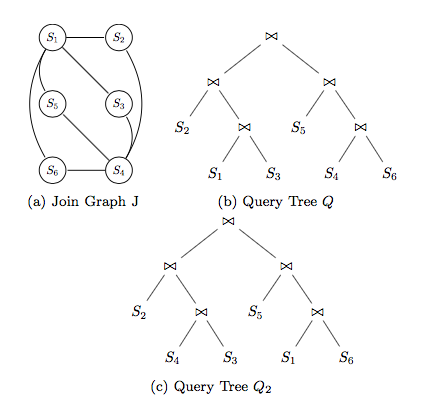
\includegraphics[width=\textwidth]{03_Related_Work/Incompleteness_RS-B2-CPS.png}
  \caption{Incompletness of RS-B2-CPS}
  \label{Incompleteness_RS-B2-CPS}
\end{figure}


\cite{shanbhag2014optimizing} stellt fest, dass RS-B0-CPS und RS-B1-CPS vollständig sind. Die Vollständigkeit von RS-B2-CPS wird jedoch in Frage gestellt und die Unvollständigkeit mit Hilfe eines Beispiels belegt. Als Beispiel dient eine Menge von Relationen, die mit Hilfe des Jointrees J (\ref{fig:Incompleteness_RS-B2-CPS}) miteinander gejoint sind. Der Initale Anfragebaum $Q1$ ist in \ref{fig:Incompleteness_RS-B2-CPS} dargestellt. Das gewünschte Ergebnis nach einer Transformation $Q2$  findet sich in \ref{fig:Incompleteness_RS-B2-CPS}. 

Bei RS-B2-CPS dürfen die Regeln R2, R3, R4 nur jeweils einmal auf einen Join-Operator angewendet werden. Keine der Regeln darf danach auf den neu generierten Operator angewendet werden. Die In \ref{fig:Q1} und \ref{fig:Q2} zeichnet sich dadurch aus, dass die Relationen $R1$ und $R4$ vertauscht sind.







\subsubsection{Vorschlag von RS-Graph}

\subsection{JOIN SETS}

Basierend auf dem bisherigen Wissen, wurden durch X und y einige neue Begriffe festgelegt:W
Ein Base Equivalence Knoten in einem expandierten LQDAG ist ein Äquivalenzknoten, der keinen Join Operator als Kinder hat. Ein solcher Knoten kann entweder eine Relation sein oder darf keine Join Operatoren als Kinder beinhalten.

Ein Join Tree ist in einem expandierten LQDAG ein Baum in der LQDAG dessen Wurzel ein Äuqivalenzknoten und jeder interne Knoten entweder ein Äquivalenzknoten oder ein Join Operator und jeder untergeordneter Knoten ein Äuqivalenzknoten ist.

Der Maximale JOIN Tree ist in einem expandierten LQDAG ein Join Tree, bei dem jeder Leaf knoten ein Base Equivalence Node ist.

Ein Join-Set für einen Äquivalenzknoten E ist in einem expandierten LQDAG ein Paar $J = (S, P)$ bei dem S ein Set von Äquivalenzknoten ist, deren 

\subsection{Ruleset RS-Graph}
Neben den bereits etablierten Regeln wird eine neue Regel für den Volcano Optimizer von \cite{shanbhag2014optimizing} vorgestellt. Die neue Transformationsregel $RS-Graph$ ersetzt die bisherigen Regeln und die bisherigen Regelsets. Die neue Regel erzeugt basierend auf einem Planknoten direkt alle möglichen äquivalenten Pläne. Somit sind alle Pläne unter einem bestimmten Äquivalenzknoten mit der Anwendung nur einer Regel erzeugt.

Die Regel $RS-Graph$ verwendet dazu die Subroutine $GraphRule$. Sie wird auf den Join Tree angewendet, falls die beiden mit einem Operator verbundenen Knoten A und B und deren Mitterknoten $P$. Für jedes Paar der J $$equivalence nodes A,B and parent equivalence node P. For each pair of join-set (jsA,jsB) ∈ A.JoinSets∗B.JoinSets, we merge the pair to form a join-set js. We define the merge of the two join-sets jsA = (V1,P1) and jsB = (V2,P2) as (V1∪V2,P1 ∧P2).$$

Um wiederholte Berechnungen des selben Join TRees zu vermeiden wird zudem geprüft, ob der Eltern-Äquivalenzknoten bereits $js$ beinhaltet. $$To check if two join- sets at an equivalence node are equal, it is sufficient to check if they have same equivalence nodes. If the join-sets have the same equivalence nodes, then they will also have the same predicates.$$

Für alle Join Sets $js$ des Parent nodes werden daraufhin zuerst alle JOIN partitionen gebildet bei denen $S_1 \Join S_2$ mit 

Sollte der $js$ noch nicht existieren, wird dieser dem JOIN Set hinzugefügt. Ein Graph wird basierend auf den $js$ gebildet, der mit Hilfe der Methode Partition in alle Partitionen getrennt wird. Aus denen wiederum Bäume erstellt werden, die an das Resultat zurückgegeben werden.

Die SubRoutine Create Graph, gibt ein JOIN Set, das JS einen Join Graphen aus, der




\subsection{Discussion}
Die Implementierung der neuen Regel wurde in einem Java basierten regelbasierten Optimierer implementiert. Dieser Optimierer “ProtoJ” ist eine Übersetzung des Optimierers Proto aus C++ in Java. Für die Implementierung mussten neue Felder den Äquivalenzklassen hinzugefügt werden.

Die Generierung der Resultate find ohne Pruning statt und kosten für die Kostenberechnung wurden nicht einbezogen. Ebenfalls bleiben Regeln bestehen, die für denn SELECT Pushdown verantwortlich sind, als teil der Normalisierungsphase. 

Es wurden sowohl Star, Chain als auch Clique Queries getestet. Die Experimente fanden auf einem Intel i5 3.5 GHz mit 8 GB Ram statt. Es wurde festgestellt, dass die Geschwindigkeit der Optimierung verbessert werden konnte, dadurch, dass die Optimierung mehrfach durchgeführt wurde. Dieses Verhalten wurde auf Javas JIT Kompilierungsstrategie zurückgeführt. Die erst den Code Kompiliert, wenn er auch tatsächlich gebraucht wird. Um sicherzustellen, dass der Kompilierte Code nicht wieder während der Ausführung vergessen geht mussten spezielle Flags für die JVM gesetzt werden. Das Ergebnis war, dass die Dauer zwar verglichen zu den schnellsten Test ohne das Flag langsamer, aber dafür konstant blieben.

Ebenfalls wurde bei Ruleset $RS_B1$ geprüft, ob der gesamte Search Space erreicht wurde, indem die Anzahl der Äquivalenten Knoten und Operatoren im LQDAG gezählt wurden. Diese Zahl wurde mit der Zahl der Knoten in RS-Graph verglichen. Da beide zahlen gleich war, wird davon ausgegangen, dass beide Regelsets das selbe Ergebnis erzeugen. Eine Prüfung, die dies belegt fand aus technischen Gründen nicht statt.






ersetzten X und Y die bisher gezeigten Regeln des Volcano Optimizers mit einer neuen Transformationsregel: RS-Graph. Die Regel kommt zur Anwendung, falls ein Graph dem Pattern $E_1 \Join E_2$ entspricht. Ist dies der Fall wird die Funktion $GraphRule(\Join, E_1, E_2, parent)$ aufgerufen. Sie erzeugt ein Set von allen Join Operatoren unter dem Equivalenzklasse des $parent$-Knotens.




\subsubsection{}



\subsection{Patition zu Graph}



Die Methode Partition gibt eine Menge von Partitionen zurück. Jede Partition bezeichnet eine Menge von Knoten. Sowohl $S_1$ als auch $G\\S_1$ sind Teil dieser Menge, falls beide zwischen beiden im Joni-Graphen miteinander verbunden sind. Im Gegensatz zu anderen Regeln, die pro Anwendung der Regel nur immer einen neuen Knoten zurückgegeben haben, gibt die neue Regel immer Bäume zurück, die alle möglichen Join Operatoren unterhalb des ROOT Operators beinhalten.
>>>>>>> 2dbe3382d95b975a93a2c2789dd91dda3468d5cc
